\documentclass[11pt,a4paper]{article}

% ---------- Packages ----------
\usepackage[margin=2.4cm]{geometry}
\usepackage{graphicx}
\usepackage{amsmath, amssymb}
\usepackage{booktabs}
\usepackage{multirow}
\usepackage{float}
\usepackage{subcaption}
\usepackage{hyperref}
\usepackage{url}
\usepackage{caption}
\usepackage{listings}
\usepackage{xcolor}
\usepackage{siunitx}

\hypersetup{
  colorlinks=true,
  linkcolor=blue,
  urlcolor=blue,
  citecolor=blue
}

% ---------- Code listing style ----------
\lstdefinestyle{mystyle}{
  basicstyle=\ttfamily\small,
  breaklines=true,
  frame=single,
  columns=fullflexible,
  keywordstyle=\color{blue},
  commentstyle=\color{gray},
  stringstyle=\color{teal},
  showstringspaces=false
}
\lstset{style=mystyle}

% ---------- Title ----------
\title{\textbf{Deep Learning for the Detection of \textit{Helicobacter pylori}\\
in Immunohistochemical Histopathological Images}\\[4pt]
\large Project-Based Learning Report}
\date{\today}

\begin{document}
% ---------- Front cover (guidelines: project name, representative image, names+NIU, UAB, course, date) ----------
\begin{titlepage}
  \centering
  \vspace*{1cm}
  {\LARGE\textbf{Deep Learning for the Detection of \textit{Helicobacter pylori}\\
  in Immunohistochemical Histopathological Images}\par}
  \vspace{0.5cm}
  {\large Project-Based Learning Report\par}
  \vspace{1.5cm}
  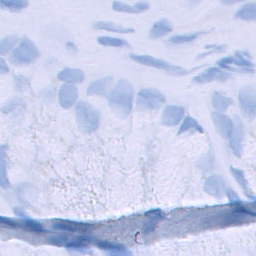
\includegraphics[width=0.7\linewidth]{figures/cover.png}\\[1cm]
  \textit{Representative histology: IHC-stained gastric biopsy patch.}
  \vfill
  \begin{tabular}{rl}
    Théotime Donnenfeld & NIU 1786565 \\
    Rubén Alba & NIU 1786494 \\
    Rohit Ranbawale & NIU 1744008 \\
    Michael Rienessl & NIU 1699828 \\
  \end{tabular}
  \vspace{1cm}\par
  Universitat Autònoma de Barcelona (UAB)\\
  \textbf{Course: Deep Learning}
  \vspace{0.5cm}\par
  \today
\end{titlepage}
\newpage

% ---------- Abstract ----------
\begin{abstract}
\noindent
We use the Quiron Salut dataset of 245 gastric biopsies (immunohistochemically stained whole-slide images) to implement and compare two patch-level models for \textit{Helicobacter pylori} detection.
A patch-based pipeline processes $256\times256$ patches extracted along tissue borders.
Two approaches are implemented: (i) a supervised convolutional neural network (CNN) trained on expert-annotated patches, and (ii) an unsupervised autoencoder (AE) trained on healthy patches and used for anomaly detection via reconstruction error.
This report shows that both models are running and have been compared on the same validation set: we evaluate them with the comparison script (\texttt{compare\_patch\_classifiers.py}), report patch-level accuracy and precision, and include a side-by-side confusion-matrix plot.
\textbf{Scope of this first report is patch-level comparison; patient-level aggregation and evaluation on the independent hold-out set are planned as next steps.}
\end{abstract}

\newpage

% ==========================================================
\section{Introduction}
\label{sec:intro}

\textit{Helicobacter pylori} is a gastric bacterium associated with chronic gastritis and an increased risk of gastric cancer. In clinical practice, detection often relies on the visual inspection of immunohistochemically (IHC) stained histopathology slides. Whole-slide images (WSI) can exceed 100\,000 pixels per side, making manual review time-consuming. This project investigates automated, patch-based detection: we classify small image patches as healthy or containing bacteria, then aggregate patch predictions to obtain a patient-level diagnosis.

The pipeline has three stages: (1) train a patch-level classifier on expert-annotated data; (2) apply it to all patches of each patient and compute the fraction of positive patches; (3) compare that fraction to a threshold to yield a binary patient diagnosis. Key challenges are the limited number of annotated patches, strong class imbalance (few patches contain bacteria), and the need to avoid data leakage by splitting at the patient level rather than the patch level.

We implement two patch-level models---a supervised CNN and an unsupervised autoencoder used for anomaly detection---and compare them on the same validation set. This report describes the methodology, experimental setup, and patch-level results; patient-level aggregation and evaluation on an independent hold-out set are left for future work.

% ==========================================================
\section{Dataset Description}
\label{sec:dataset}

We use the Quiron Salut dataset: IHC-stained gastric biopsy whole-slide images from which $256\times256$ pixel patches have been cropped along the tissue border. Patient-level labels indicate H.\textit{ pylori} density: NEGATIVE, LOW, or HIGH. For binary classification we map NEGATIVE to 0 and (LOW, HIGH) to 1.

Patch-level annotations are provided in \texttt{CoordAnnotatedAllPatches.csv} with a \texttt{Presence} field: $-1$ (healthy), $1$ (bacteria present), or $0$ (unclear, excluded from training).

The data are organised into three parts: \textbf{CrossValidation/Annotated} (expert-labelled patches for training and validating patch-level models), \textbf{CrossValidation/Cropped} (all patches per patient for aggregation experiments), and \textbf{HoldOut} (116 independent patients reserved for final evaluation only). Table~\ref{tab:dataset_stats} summarises the sample counts.

\begin{table}[H]
\centering
\begin{tabular}{lcccc}
\toprule
Split & \#Patients & \#Annotated patches & \#Positive patches & \#Negative patches \\
\midrule
CrossValidation & 123 & 1211 & 161 & 1050 \\
HoldOut & 116 & -- & -- & -- \\
\bottomrule
\end{tabular}
\caption{Dataset size overview (Quiron Salut).}
\label{tab:dataset_stats}
\end{table}

% ==========================================================
\section{Methodology}
\label{sec:methodology}

\subsection{Pipeline overview}
The pipeline has three steps.
First, a patch-level model (CNN or autoencoder) is trained on annotated or healthy-only patches. Second, the model is applied to every patch of each patient. Third, the fraction of patches predicted positive per patient is computed and compared to a threshold $\tau_{patient}$ to obtain a binary patient-level diagnosis. Within this first report we address patch-level classification by comparing an autoencoder and a CNN classifier. Figure~\ref{fig:methodology} summarises the workflow.

\begin{figure}[H]
\centering
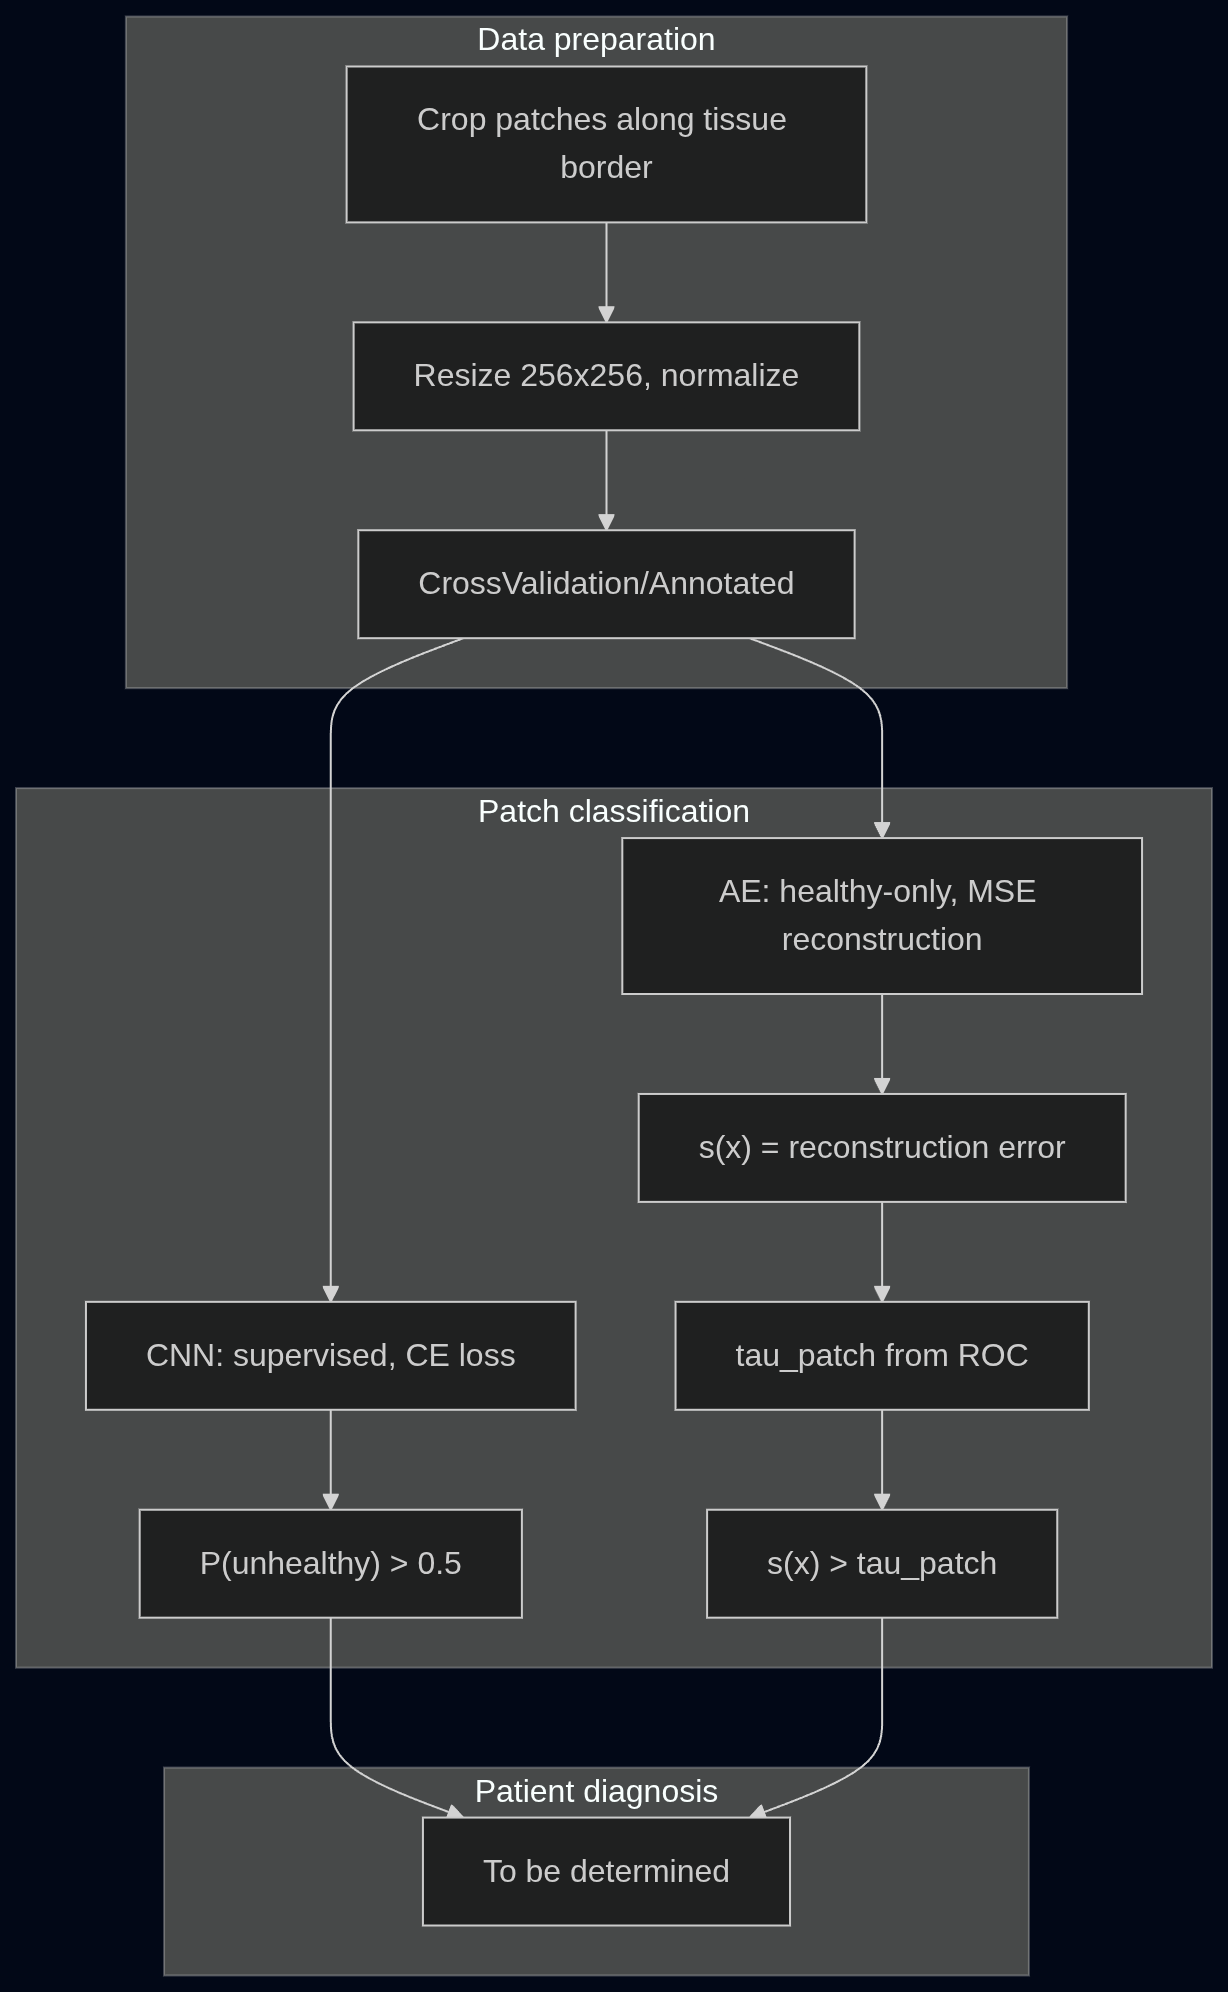
\includegraphics[width=\linewidth]{figures/methodology.png}
\caption{Methodology workflow: data preparation, patch-level classification (CNN vs autoencoder), and patient-level aggregation (to be evaluated in a later phase).}
\label{fig:methodology}
\end{figure}

\subsection{Preprocessing}
Patches are loaded as RGB images, resized to $256\times256$ if needed, and normalised per channel with $x' = (x - \mu)/\sigma$ where $\mu = \sigma = (0.5, 0.5, 0.5)$, so that inputs lie approximately in $[-1, 1]$. For the CNN we apply data augmentation: random flips, small rotations, and optional colour jitter.

\subsection{Patch-level approach 1: CNN classifier}
We use a lightweight CNN with three convolutional blocks followed by fully connected layers. Training minimises cross-entropy loss. With one-hot label $y$ and predicted class probabilities $\hat{p}_c$ (softmax over logits), the loss is
\[
\mathcal{L}_{\mathrm{CE}} = -\sum_{c \in \{0,1\}} y_c \log \hat{p}_c,
\]
with $c=0$ for healthy and $c=1$ for patches containing H.\textit{ pylori}. The model is trained with Adam; early stopping is optional. At inference, a patch is predicted positive if the probability of class 1 exceeds 0.5.

\subsection{Patch-level approach 2: Autoencoder anomaly detection}
The autoencoder is trained only on healthy patches and learns to reconstruct normal tissue. Training minimises mean squared error between input and reconstruction:
\[
\mathcal{L}_{\mathrm{AE}} = \frac{1}{CHW} \sum_{c,i,j} (x_{c,i,j} - \hat{x}_{c,i,j})^2,
\]
where $C=3$, $H=W=256$. The per-patch anomaly score $s(x)$ is the reconstruction error. We use either the mean over all pixels or the maximum over $8\times8$ spatial cell means (\texttt{max\_local}) so that small anomalous regions contribute more. A patch is predicted positive if $s(x) > \tau_{patch}$. The threshold $\tau_{patch}$ is chosen on the validation set as the point on the ROC curve closest to (FPR$=0$, TPR$=1$), implemented as \texttt{roc\_threshold\_optimal}.

\subsection{Patient-level aggregation}
For each patient $p$ with $N_p$ patches and binary patch predictions $\hat{z}_i \in \{0,1\}$, we define the contamination ratio $r_p = \frac{1}{N_p}\sum_{i=1}^{N_p} \hat{z}_i$. The patient is predicted positive if $r_p > \tau_{patient}$. Both $\tau_{patch}$ and $\tau_{patient}$ are selected using cross-validation data only and held fixed for hold-out evaluation.

% ==========================================================
\section{Implementation Details}
\label{sec:implementation}

\subsection{Development iterations}
The CNN started as a minimal classifier: three small convolutional blocks (3$\to$16$\to$32$\to$64 channels, ReLU, max pooling) and two fully connected layers mapping the flattened 64$\times$32$\times$32 features to two class logits. No architectural changes were required for good performance; the main refinements were patient-level train/validation splitting to avoid leakage, ignoring patches with \texttt{Presence=0} in the annotation file, and training for more epochs (e.g.\ 150 in the Slurm script). The current design remains lightweight and fast to train.

The autoencoder began with a shallower encoder (32$\to$64$\to$128$\to$256$\to$256 channels, 8$\times$8 bottleneck) and ReLU activations. To avoid losing information in the bottleneck (ReLU zeros negatives), ReLU was replaced by LeakyReLU. The encoder and decoder were then deepened and widened (64$\to$128$\to$256$\to$512$\to$512 channels, 8$\times$8$\times$512 bottleneck) to improve reconstruction of healthy tissue so that anomalous patches yield higher error. The anomaly score was extended with a \texttt{max\_local} option (maximum over $8\times8$ spatial cell means) so that focal H.\textit{ pylori} regions drive the score. Checkpoint selection was fixed to keep the best model by validation loss instead of the last epoch, and the default aggregation and epoch count were set to \texttt{max\_local} and 35 (overridable via Slurm).

\subsection{Code structure}
The codebase is organised as follows: \texttt{model.py} defines and trains the CNN; \texttt{model\_autoencoder.py} defines and trains the autoencoder and implements ROC-based threshold selection; \texttt{compare\_patch\_classifiers.py} loads both checkpoints, runs them on the same validation loader, and saves the confusion-matrix and ROC figures. Training on a GPU cluster is launched via \texttt{train.sbatch.sh} and \texttt{train\_autoencoder.sbatch.sh}. Dataset paths follow the \texttt{HelicoDataSet/} layout (CrossValidation/Annotated, HoldOut). Key code snippets---the comparison loop, CNN architecture, AE reconstruction error and threshold selection, patient-level aggregation pseudocode, and Slurm commands---are gathered in Appendix~\ref{app:code} (Listings~\ref{lst:compare}--\ref{lst:slurm}). Reproducibility is ensured by fixed random seeds, a fixed patient-level split, and logging of hyperparameters and checkpoints.

% ==========================================================
\section{Experimental Design}
\label{sec:experiments}

We split the Cross-Validation set at the \textbf{patient level}: every patch of a given patient is assigned to either training or validation, never both, to avoid leakage. A single random split is used with 80\% of patients for training and 20\% for validation (\texttt{val\_ratio=0.2}, \texttt{seed=1}), and the same split is used in \texttt{model.py}, \texttt{model\_autoencoder.py}, and \texttt{compare\_patch\_classifiers.py} so that both models are evaluated on identical validation patches. For full reporting we intend to use $k$-fold cross-validation over patients; the results below correspond to this single split. The Hold-out set (116 patients) is reserved for a single final evaluation after all thresholds have been fixed on cross-validation data.

We report confusion matrices and, at patch and patient level, accuracy, precision, recall, specificity, and F1. When multiple folds are available we will add confidence intervals and paired statistical tests (e.g.\ Wilcoxon) between the two methods. Hyperparameters are summarised in Table~\ref{tab:hparams}.

\subsection{Hyperparameters}
\begin{table}[H]
\centering
\begin{tabular}{ll}
\toprule
Hyperparameter & Value \\
\midrule
Optimizer & Adam \\
Learning rate & $10^{-3}$ \\
Batch size & 32 \\
Epochs (CNN) & 150 \\
Epochs (AE) & 150 \\
Weight decay & 0 (not used) \\
Early stopping & not used \\
Train/val split & patient-level, \texttt{val\_ratio=0.2}, \texttt{seed=1} \\
Patch threshold $\tau_{patch}$ & ROC: $\arg\min_\tau \bigl(\mathrm{FPR}(\tau)^2 + (1 - \mathrm{TPR}(\tau))^2\bigr)$ (\texttt{roc\_threshold\_optimal}) \\
Patient threshold $\tau_{patient}$ & from CV; hold-out evaluation TBD \\
\bottomrule
\end{tabular}
\caption{Hyperparameters and training configuration (from \texttt{model.py}, \texttt{model\_autoencoder.py}, and Slurm scripts).}
\label{tab:hparams}
\end{table}

% ==========================================================
\section{Results}
\label{sec:results}

Both models were evaluated on the same validation fold: 115 training patients (1889 patches) and 28 validation patients (730 patches, of which 419 are healthy and 311 contain H.\textit{ pylori}). We used the checkpoints \texttt{models/classifier/best\_model.pth} (CNN) and \texttt{models/autoencoder/autoencoder\_model.pth} (AE). Patch-level metrics are given in Table~\ref{tab:patch_results}; Figure~\ref{fig:compare_confusion} shows the confusion matrices and Figure~\ref{fig:roc} the ROC curves. Patient-level results (Table~\ref{tab:patient_results}) will be filled after aggregation and hold-out evaluation.

\subsection{Patch-level metrics}
Table~\ref{tab:patch_results} summarises patch-level performance. Recall is TP/(TP+FN) and specificity is TN/(TN+FP). The CNN attains higher accuracy and precision; the autoencoder is slightly lower but still strong, and was trained without any positive patch labels.
\begin{table}[H]
\centering
\begin{tabular}{lcccc}
\toprule
Method & Accuracy & Precision & Recall & Specificity \\
\midrule
CNN & 0.989 & 0.978 & 0.997 & 0.983 \\
Autoencoder & 0.959 & 0.940 & 0.965 & 0.955 \\
\bottomrule
\end{tabular}
\caption{Patch-level performance on the validation fold (730 patches).}
\label{tab:patch_results}
\end{table}

\subsection{Confusion matrices and ROC}
Figure~\ref{fig:compare_confusion} shows the confusion matrices for the same 730 validation patches. For the CNN (left), with threshold 0.5 on the positive-class probability, we obtain TN=412, FP=7, FN=1, TP=310. For the autoencoder (right), with $\tau_{patch}$ chosen on the validation ROC (closest to (FPR=0, TPR=1)), we obtain TN=400, FP=19, FN=11, TP=300. Figure~\ref{fig:roc} displays the ROC curves for both methods.
\begin{figure}[H]
\centering
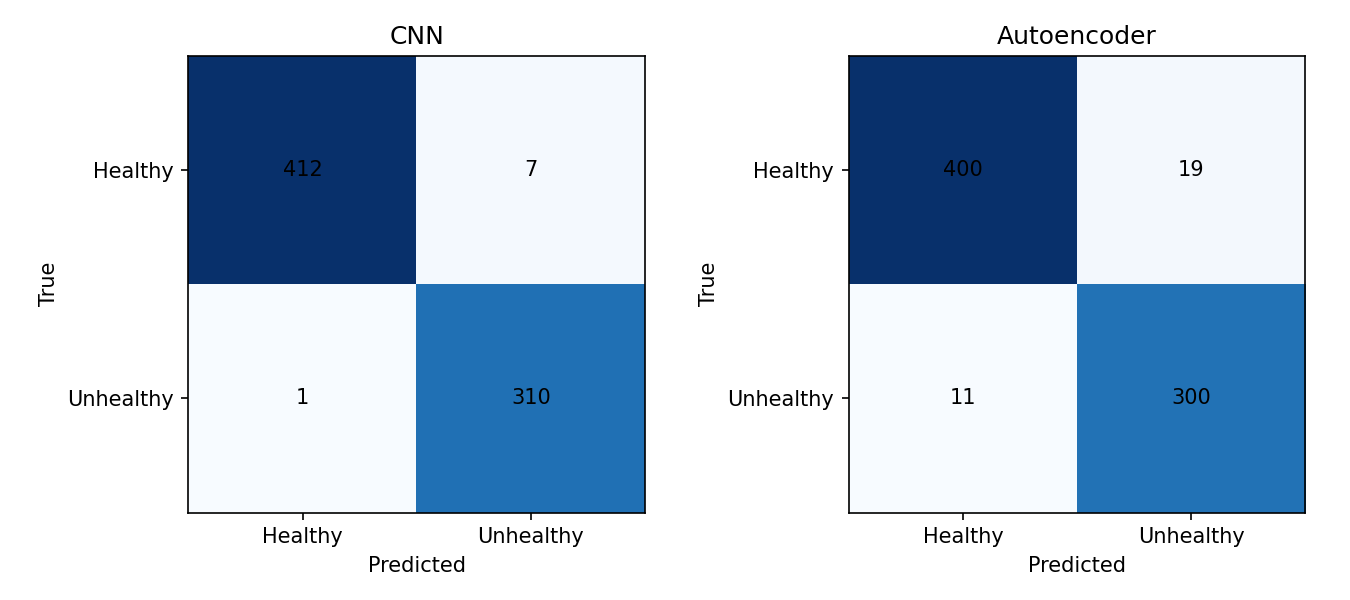
\includegraphics[width=0.9\linewidth]{figures/compare_confusion.png}
\caption{Confusion matrices on the validation set. Left: CNN. Right: Autoencoder (threshold from validation ROC).}
\label{fig:compare_confusion}
\end{figure}
\begin{figure}[H]
\centering
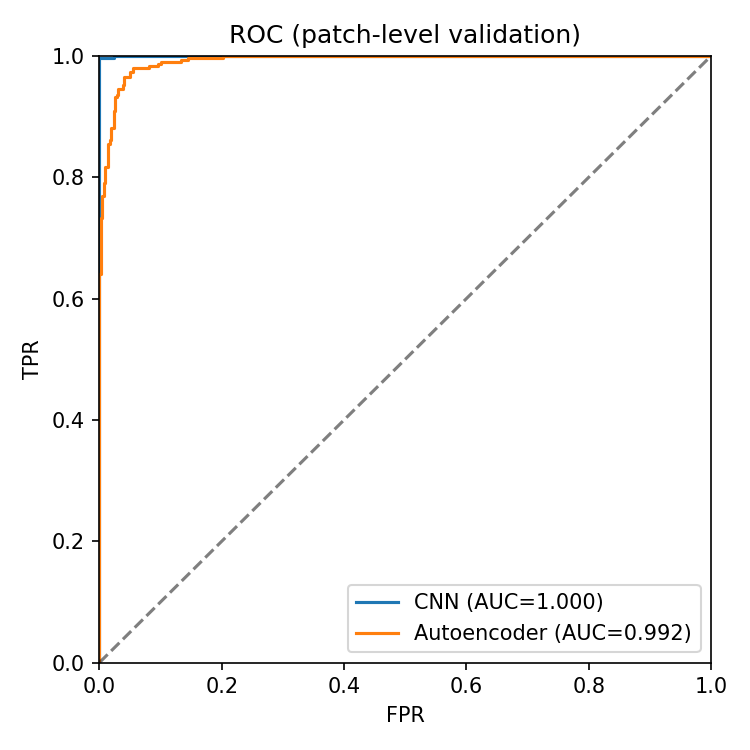
\includegraphics[width=0.75\linewidth]{figures/compare_roc.png}
\caption{ROC curves on the validation set.}
\label{fig:roc}
\end{figure}

\subsection{Patient-level}
Patient-level performance (after aggregating patch predictions per patient and applying $\tau_{patient}$) will be reported once thresholds are fixed and the hold-out set is evaluated (Table~\ref{tab:patient_results}).
\begin{table}[H]
\centering
\begin{tabular}{lcccc}
\toprule
Method & Accuracy & Precision & Recall & Specificity \\
\midrule
CNN + aggregation & -- & -- & -- & -- \\
AE + aggregation & -- & -- & -- & -- \\
\bottomrule
\end{tabular}
\caption{Patient-level performance (to be filled after aggregation and hold-out evaluation).}
\label{tab:patient_results}
\end{table}

% ==========================================================
\section{Discussion}
\label{sec:discussion}

On the validation fold, the CNN achieves higher accuracy (0.989) and precision (0.978) than the autoencoder (0.959 and 0.940), with fewer false positives (7 vs.\ 19) and false negatives (1 vs.\ 11). The supervised model thus benefits from seeing both healthy and positive examples during training. The autoencoder, trained only on healthy patches, remains competitive and avoids the need for positive patch labels, which is attractive when annotations are scarce or imbalanced. Both models achieve high recall (0.997 and 0.965), which is desirable in a screening context where missing a positive case is costly.

The main limitations of the current evaluation are the use of a single train/validation split (so that confidence intervals and statistical tests are not yet available), the limited number of annotated patches, and possible variability in staining and scanning across slides. The threshold-based aggregation from patches to patients could be refined using multiple-instance learning (e.g.\ attention-based pooling). Planned next steps include $k$-fold cross-validation with CIs and paired tests, patient-level aggregation and threshold selection, hold-out evaluation, and optionally stain normalisation and MIL for patient-level diagnosis.

% ==========================================================
\section{Conclusion}
\label{sec:conclusion}
We implemented two patch-level models for H.\textit{ pylori} detection in IHC gastric biopsy images: a supervised CNN and an unsupervised autoencoder for anomaly detection. Both were trained on the Quiron Salut dataset and evaluated on the same validation set (730 patches from 28 patients). The CNN reaches 0.989 accuracy and 0.978 precision; the autoencoder reaches 0.959 and 0.940 without using positive patch labels at training time. We reported the methodology, implementation details, patch-level metrics, confusion matrices, and ROC curves. The next steps are $k$-fold cross-validation with statistical comparison, patient-level aggregation, and evaluation on the independent hold-out set.


\newpage

% ==========================================================
\section*{References}
\addcontentsline{toc}{section}{References}
\begin{enumerate}
  \item Anomaly detection via reconstruction: \url{https://arxiv.org/abs/2309.16053} (self-supervised / generative models for small sample size).
\end{enumerate}

% ==========================================================
\appendix
\section{Code extracts}
\label{app:code}

\begin{lstlisting}[language=Python, caption={Comparison script: both models on the same validation set (\texttt{compare\_patch\_classifiers.py}).},label=lst:compare]
    # CNN
    cnn = SimpleCNN(num_classes=2).to(device)
    cnn.load_state_dict(torch.load(args.cnn_checkpoint, ...))
    cnn_probs, labels = compute_cnn_probs(cnn, val_loader, device)
    cnn_pred = (cnn_probs >= 0.5).astype(np.int64)

    # Autoencoder
    ae = PatchAutoencoder().to(device)
    ae.load_state_dict(torch.load(args.ae_checkpoint, ...))
    ae_errors, ae_labels = compute_reconstruction_errors(ae, val_loader, device, ...)
    ae_pred = (ae_errors > ae_threshold).astype(np.int64)

    acc_cnn, prec_cnn, cm_cnn = _metrics(labels, cnn_pred)
    acc_ae, prec_ae, cm_ae = _metrics(labels, ae_pred)
\end{lstlisting}

\begin{lstlisting}[language=Python, caption={CNN for patch classification (\texttt{model.py}).},label=lst:cnn]
class SimpleCNN(nn.Module):
    def __init__(self, num_classes: int = 2) -> None:
        super().__init__()
        self.features = nn.Sequential(
            nn.Conv2d(3, 16, 3, padding=1), nn.ReLU(), nn.MaxPool2d(2),
            nn.Conv2d(16, 32, 3, padding=1), nn.ReLU(), nn.MaxPool2d(2),
            nn.Conv2d(32, 64, 3, padding=1), nn.ReLU(), nn.MaxPool2d(2),
        )
        self.classifier = nn.Sequential(
            nn.Flatten(), nn.Linear(64 * 32 * 32, 128), nn.ReLU(),
            nn.Linear(128, num_classes),
        )
    def forward(self, x): return self.classifier(self.features(x))
\end{lstlisting}

\begin{lstlisting}[language=Python, caption={Autoencoder: Encoder, Decoder, and full model (\texttt{model\_autoencoder.py}).},label=lst:ae]
class Encoder(nn.Module):
    def __init__(self):
        super().__init__()
        self.conv = nn.Sequential(
            nn.Conv2d(3, 64, 3, padding=1), nn.LeakyReLU(0.2), nn.MaxPool2d(2),
            nn.Conv2d(64, 128, 3, padding=1), nn.LeakyReLU(0.2), nn.MaxPool2d(2),
            nn.Conv2d(128, 256, 3, padding=1), nn.LeakyReLU(0.2), nn.MaxPool2d(2),
            nn.Conv2d(256, 512, 3, padding=1), nn.LeakyReLU(0.2), nn.MaxPool2d(2),
            nn.Conv2d(512, 512, 3, padding=1), nn.LeakyReLU(0.2), nn.MaxPool2d(2),
        )
    def forward(self, x): return self.conv(x)

class Decoder(nn.Module):
    def __init__(self):
        super().__init__()
        self.up = nn.Sequential(
            nn.ConvTranspose2d(512, 512, 2, stride=2), nn.LeakyReLU(0.2),
            nn.ConvTranspose2d(512, 256, 2, stride=2), nn.LeakyReLU(0.2),
            nn.ConvTranspose2d(256, 128, 2, stride=2), nn.LeakyReLU(0.2),
            nn.ConvTranspose2d(128, 64, 2, stride=2), nn.LeakyReLU(0.2),
            nn.ConvTranspose2d(64, 3, 2, stride=2), nn.Tanh(),
        )
    def forward(self, x): return self.up(x)

class PatchAutoencoder(nn.Module):
    def __init__(self):
        super().__init__()
        self.encoder = Encoder()
        self.decoder = Decoder()
    def forward(self, x):
        return self.decoder(self.encoder(x))
\end{lstlisting}

\begin{lstlisting}[language=Python, caption={AE per-sample reconstruction error (\texttt{model\_autoencoder.py}). \texttt{mean}: pixel MSE; \texttt{max\_local}: max over 8$\times$8 cell means.},label=lst:ae_error]
def reconstruction_error_per_sample(model, x, aggregation="mean"):
    x_hat = model(x)
    err = (x - x_hat).pow(2).mean(dim=1, keepdim=True)  # (B, 1, H, W)
    if aggregation == "mean":
        return err.view(x.size(0), -1).mean(dim=1)
    if aggregation == "max_local":
        B, _, H, W = err.shape
        cell = 8
        nc_h, nc_w = H // cell, W // cell
        err = err.view(B, 1, nc_h, cell, nc_w, cell).mean(dim=(3, 5))
        return err.view(B, -1).max(dim=1)[0]
\end{lstlisting}

\begin{lstlisting}[language=Python, caption={ROC-based patch threshold: closest to (FPR=0, TPR=1) (\texttt{roc\_threshold\_optimal}, \texttt{model\_autoencoder.py}).},label=lst:roc]
def roc_threshold_optimal(errors, labels, positive_class=1):
    order = np.argsort(-errors)
    sorted_errors, sorted_labels = errors[order], (labels[order] == positive_class).astype(np.float64)
    n_pos, n_neg = sorted_labels.sum(), len(sorted_labels) - n_pos
    tpr = np.cumsum(sorted_labels) / n_pos
    fpr = np.cumsum(1.0 - sorted_labels) / n_neg
    thresh = np.concatenate([[sorted_errors[0]+1], sorted_errors, [sorted_errors[-1]-1]])
    thresh = (thresh[:-1] + thresh[1:]) / 2
    dist = fpr**2 + (1 - tpr)**2
    idx = np.argmin(dist)
    return float(thresh[idx]), float(tpr[idx]), float(fpr[idx])
\end{lstlisting}

\begin{lstlisting}[language=Python, caption={Patient-level aggregation.},label=lst:aggregation]
for patient in patients:
    patches = load_all_cropped_patches(patient)
    patch_scores = [model_score(p) for p in patches]  # CNN prob or AE error
    contaminated = [1 if s > tau_patch else 0 for s in patch_scores]
    ratio = sum(contaminated) / len(contaminated)
    patient_pred = 1 if ratio > tau_patient else 0
\end{lstlisting}

\begin{lstlisting}[language=bash, caption={Slurm training and comparison commands.},label=lst:slurm]
sbatch train.sbatch.sh
sbatch train_autoencoder.sbatch.sh
python compare_patch_classifiers.py
\end{lstlisting}

\end{document}
